\subsection{UC6: Ricerca dei prodotti}
\label{sec:UC6}
\begin{figure}[!ht]
    \caption{Diagramma di UC6: Ricerca dei prodotti}
    \vspace{10px}
    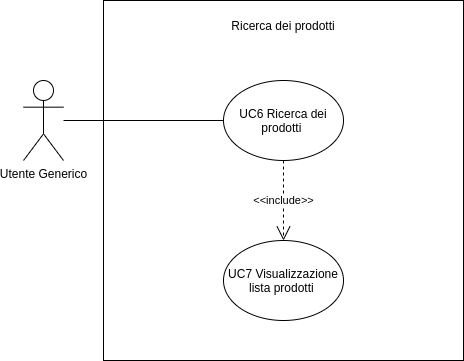
\includegraphics[scale=0.5]{../../../Images/AnalisiRequisiti/UC06}
    \centering
\end{figure}
\begin{itemize}
    \item \textbf{Descrizione:} l'utente vuole ricercare un prodotto in base ad una parola chiave;
    \item \textbf{Attore Primario:} utente non autenticato;
    \item \textbf{Precondizione:} l'utente si trova in una pagina dedicata alla ricerca;
    \item \textbf{Input:} stringa relativa a ciò che si vuole cercare;
    \item \textbf{Postcondizione:} l'utente visualizza i prodotti corrispondenti alla parola chiave (\hyperref[sec:UC7]{\underline{UC7}});
    \item \textbf{Scenario Principale:}
          \begin{itemize}
              \item l'utente vuole ricercare un prodotto secondo una determinata parola chiave;
              \item gli vengono mostrati tutti i risultati della ricerca nella lista dei prodotti.
          \end{itemize}
    \item \textbf{Inclusioni:}
          \begin{itemize}
              \item viene visualizzata una pagina con tutti i risultati della ricerca.
          \end{itemize}
\end{itemize}
